\chapter*{即値代入の制限における規則性}
\section{実験の目的}
\aasm の{\ttfamily mov}命令\footnote{レジスタに即値,またはレジスタの値を代入する命令.}は,\iasm で扱った{\ttfamily mov}命令と対応する.しかし,\aasm の{\ttfamily mov}命令において,レジスタに代入できる即値には制限がある.本実験の目的は,その制限について実験に基づき示すことである.\par
\section{実験の方法}
コンピュータ(\ref{src:usingpc})を利用して,{\ttfamily mov.s}(\ref{src:mov})ファイルをアセンブルする.
\begin{lstlisting}[caption={利用コンピュータ及び実行環境},label={src:usingpc},language={Bash},numbers={none},breakindent={0pt}]
$ uname -a
Linux KUT20VLIN-322 5.4.0-70-generic #78~18.04.1-Ubuntu SMP Sat Mar 20 14:10:07 UTC 2021 x86_64 x86_64 x86_64 GNU/Linux
$ arm-none-eabi-as --version
GNU assembler (2,27-9ubuntu1+9) 2.27
$ bash --version
GNU bash, バージョン 4.4.20(1)-release (x86_64-pc-linux-gnu)
\end{lstlisting}
\begin{tabular}[c]{cc}
    \begin{minipage}[t]{0.45\textwidth}
        \centering
        \begin{lstlisting}[caption={アセンブル},label={src:assmeble},language={Bash},frame={left}]
$ arm-none-eabi-as mov.s -o mov.o
$ arm-none-eabi-ld mov.o -o mov
$ ./mov ; echo $?
3
    \end{lstlisting}
        \begin{flushleft}
            \ref{src:assmeble}: 4行目は,\ref{src:mov}: 5行目のテスト値を出力する.
        \end{flushleft}
    \end{minipage} &
    \begin{minipage}[t]{0.45\textwidth}
        \centering
        \begin{lstlisting}[caption={{\ttfamily mov.s}},label={src:mov},frame={left}]
    .section    .text
    .global     _start
_start:
    mov r7, #1
    mov r0, #3 @ test number
    swi #0
\end{lstlisting}
    \end{minipage}
    \vspace{0.5em}                                                                          \\
    \begin{minipage}[c]{0.45\textwidth}
        アセンブル(\ref{src:assmeble})の際に\ref{src:error}の出力が得られた場合は,\ref{src:mov}: 5行目に問題があり即値の代入に失敗している.
    \end{minipage}
    \hspace{1em}                                                                          &
    \begin{minipage}[c]{0.45\textwidth}
        \begin{lstlisting}[numbers={none},caption={Error出力},label={src:error},frame={single}]
mov.s: Assembler messages:
mov.s:5: Error: invalid constant (4d1) after fixup
    \end{lstlisting}
    \end{minipage}
\end{tabular}
様々なテスト値を簡単に試すためにスクリプトファイルによる自動実行プログラム(\ref{src:test})を作成し,実行した\footnote{実行するに際して,空ファイル{\ttfamily test.s}を作成し,{\ttfamily mov.s}の一部を変更する必要がある.}(\ref{src:testexec}).
テストする即値は,\(1\leq N\leq 266240\)である.実行結果には,アセンブルできた即値とその即値の前にアセンブルできた即値との差(前項との差)が出力される.\par
手入力での実験に関しては,実験したい数値\(n\)を\ref{src:mov}: 5行目の {\ttfamily mov r0, \#n}と入力し,アセンブルする.
\begin{center}
    \begin{minipage}[t]{0.34\textwidth}
        \centering
        \begin{lstlisting}[caption={{\ttfamily mov.s}変更後},label={src:mov2},frame={left}]
    .equ    N,  %d
    .section    .text
    .global     _start
_start:
    mov r7, #1
    mov r0, #N @ test number
    swi #0
    \end{lstlisting}
        \begin{lstlisting}[language={Bash},numbers={none},caption={実行},label={src:testexec},frame={leftline}]
$ bash test.sh          
    \end{lstlisting}
    \end{minipage}
    \hspace{2em}
    \begin{minipage}[t]{0.58\textwidth}
        \centering
        \begin{lstlisting}[language={Bash},caption={{\ttfamily test.sh}},label={src:test},frame={left}]
#!/bin/bash
W=0
for i in 'seq 0 266240'
do
sed -e "s/%d/$i/g" mov.s > test.s
arm-none-eabi-as test.s -o test.o > /dev/null 2>&1
if [ $? -eq 0]; then
    echo "$i, OK, $(( $i - $W ))"
    V=$i
    W-$i
fi
done
    \end{lstlisting}
    \end{minipage}
\end{center}
\section{実験結果}
実験結果を\ref{tbl:実験結果シェル},\ref{tbl:実験結果手入力}に示す.\(N(n)\)は32ビットの\(n\)をビット反転させた数値である.
\begin{table}[H]
    \centering
    \begin{minipage}[t]{0.45\textwidth}
        \centering
        \caption{実験結果(シェルスクリプト)}
        \label{tbl:実験結果シェル}
        \scalebox{0.8}{
            \begin{tabular}{lccc}
                \multicolumn{2}{c}{入力数値} & アセンブルの可否     & \multicolumn{1}{c}{前項との差}          \\
                \hline
                0                        &              & OK                        & -      \\
                1                        &              & OK                        & 1      \\
                2                        &              & OK                        & 1      \\
                \vdots                   &              & \vdots                    & \vdots \\
                256                      & \((2^8)\)    & OK                        & 1      \\
                260                      &              & OK                        & 4      \\
                \vdots                   &              & \vdots                    & \vdots \\
                1024                     & \((2^{10})\) & OK                        & 4      \\
                1040                     &              & OK                        & 16     \\
                \vdots                   &              & \vdots                    & \vdots \\
                4096                     & \((2^{12})\) & OK                        & 16     \\
                4160                     &              & OK                        & 64     \\
                \vdots                   &              & \vdots                    & \vdots \\
                16384                    & \((2^{14})\) & OK                        & 64     \\
                16640                    &              & OK                        & 256    \\
                \vdots                   &              & \vdots                    & \vdots \\
                65536                    & \((2^{16})\) & OK                        & 256    \\
                66560                    &              & OK                        & 1024   \\
                \vdots                   &              & \vdots                    & \vdots \\
                262144                   & \((2^{18})\) & OK                        & 1024   \\
                266240                   &              & OK                        & 4096   \\
                \hline
            \end{tabular}
        }
    \end{minipage}
    \begin{minipage}[t]{0.45\textwidth}
        \centering
        \caption{実験結果(手入力)}
        \label{tbl:実験結果手入力}
        \scalebox{0.8}{
            \begin{tabular}{lc}
                \multicolumn{1}{c}{入力数値} & アセンブルの可否 \\
                \hline
                {\ttfamily 0x7fffff}     & MISS     \\
                {\ttfamily 0xfffffe}     & MISS     \\
                {\ttfamily 0xffffff}     & OK       \\
                \(N(2^{8})\)             & OK       \\
                \(N(2^{10})\)            & OK       \\
                \(N(2^{14})\)            & OK       \\
                \(N(0)\)                 & OK       \\
                \hline
            \end{tabular}
        }
        \begin{flushleft}
            \ref{tbl:実験結果シェル}を入力数値\(n\in\{0\}\cup\mathbb{Z_+}\)に対して,アセンブルの可能条件を一般化する.
            \begin{tcolorbox}[
                    enhanced,
                    title={\bfseries \hypertarget{kisoku1}{規則 1}},
                    boxed title style={skin=enhancedfirst jigsaw,arc=1mm,bottom=0mm,boxrule=0mm},
                    sharp corners=northwest,
                    arc=1mm,
                    attach boxed title to top left={yshift=-.5mm},
                    colframe=gray!80,
                    colbacktitle=gray!80,
                ]
                \begin{align*}
                    2^p< n\leq 2^{p+2} &    & (p=2k+6)
                    \intertext{となる\(k(1\leq k\leq 5)\)に対して,}
                    n\bmod 4^k         & =0
                \end{align*}
                であることが,\(n\)をアセンブルできる条件である.
            \end{tcolorbox}
        \end{flushleft}
    \end{minipage}
\end{table}
\section{考察}
\newcommand{\kisokua}{\hyperlink{kisoku1}{\bfseries 規則1}}
\paragraph{結果からの考察}\ref{tbl:実験結果シェル}より,{\ttfamily mov}命令による18ビットまでの即値の代入に関しては\kisokua に従っていることが判る.
さらに,入力数値のビット列が8ビットに収まり,その8ビットに収まったビット列の先頭と,レジスタの1ビット目との距離が2の倍数である必要がある(\ref{fig:exec}).\par
\paragraph{条件の推測} \ref{fig:exec},\ref{fig:exec2}より,入力数値に対して右に\(2n(n<16)\)回ローテートし,上位24ビットが全て同じ数値であれば{\ttfamily mov}命令での即値代入が可能であると推測した.
\ref{tbl:実験結果手入力}より,入力数値\(i\)が{\ttfamily 0xFFFFFF}より大きい場合,\(N(i)\)が\kisokua に準拠するならばアセンブル可能であることが予想される(\ref{fig:exec2}).\par
従って,入力数値\(n\in\{0\}\cup\mathbb{Z_+}\)に対して,アセンブルの可能条件は以下のようになることが予想される.
\begin{tcolorbox}[
        enhanced,
        title={\bfseries 規則},
        boxed title style={skin=enhancedfirst jigsaw,arc=1mm,bottom=0mm,boxrule=0mm},
        sharp corners=northwest,
        arc=1mm,
        attach boxed title to top left={yshift=-.5mm},
        colframe=black,
        colbacktitle=black,
    ]
    \begin{equation}
        n' =\left\{
        \begin{aligned}
            n    &  & (0\leq n<2^{24})        \\
            N(n) &  & (2^{24}\leq n<2^{31}-1)
        \end{aligned}
        \right.
    \end{equation}
    \tcblower
    \begin{align*}
        2^p< n'\leq 2^{p+2} &    & (p=2k+6)
        \intertext{となる\(k(1\leq k\leq 5)\)に対して,}
        n'\bmod 4^k         & =0
    \end{align*}
    であることが,\(n\)をアセンブルできる条件である.
\end{tcolorbox}
\begin{figure}[h]
    \caption{アセンブル可能な即値の例1}
    \label{fig:exec}
    \begin{center}
        \begin{tikzpicture}
            \fill[fill=magenta!10,opacity=.5](4,0)rectangle(8,1);
            \draw[thick](4,0)rectangle(8,1);
            \draw (0,0) rectangle (16,1);
            \foreach \u in {0.5,1.0, ..., 16.0}
            \draw (\u,0)--(\u,0.2);
            \foreach \u in {0.5,1.0, ..., 16.0}
            \draw (\u,1)--(\u,0.8);
            \foreach \u in {4.25,5.25,6.75,7.75}
            \node at (\u,0.5){{\ttfamily 1}};
            \foreach \u in {4.75,5.75,6.25,7.25}
            \node at (\u,0.5){{\ttfamily 0}};
            \foreach \u in {0.25,0.75,...,3.75}
            \node at (\u,0.5){{\ttfamily 0}};
            \foreach \u in {0,1,...,31}
                {
                    \node[above] at (16 - 0.25 - \u * 0.5 ,1){\scriptsize\ttfamily \u};
                }
            \foreach \u in {15.75,15.25,...,8.25}
            \node at (\u,0.5){{\ttfamily 0}};
            \draw[latex-latex,thick](8,-0.5)--(16,-0.5)node[midway,fill=white]{\scriptsize 2の倍数ビット};
            \draw[dashed](8,0)--(8,-1);
            \draw[dashed](16,0)--(16,-1);
            \node[below] at ($(4,0)!0.5!(8,0)$){\scriptsize 8ビットに収まっている};
        \end{tikzpicture}
    \end{center}
    \vspace{-1em}
    \caption{アセンブル可能な即値の例2}
    \label{fig:exec2}
    \begin{center}
        \begin{tikzpicture}
            \fill[fill=magenta!10,opacity=.5](4,0)rectangle(8,1);
            \draw[thick](4,0)rectangle(8,1);
            \draw (0,0) rectangle (16,1);
            \foreach \u in {0.5,1.0, ..., 16.0}
            \draw (\u,0)--(\u,0.2);
            \foreach \u in {0.5,1.0, ..., 16.0}
            \draw (\u,1)--(\u,0.8);
            \foreach \u in {4.25,5.25,6.75,7.75}
            \node at (\u,0.5){{\ttfamily 0}};
            \foreach \u in {4.75,5.75,6.25,7.25}
            \node at (\u,0.5){{\ttfamily 1}};
            \foreach \u in {0.25,0.75,...,3.75}
            \node at (\u,0.5){{\ttfamily 1}};
            \foreach \u in {0,1,...,31}
                {
                    \node[above] at (16 - 0.25 - \u * 0.5 ,1){\scriptsize\ttfamily \u};
                }
            \foreach \u in {15.75,15.25,...,8.25}
            \node at (\u,0.5){{\ttfamily 1}};
            \draw[latex-latex,thick](8,-0.5)--(16,-0.5)node[midway,fill=white]{\scriptsize 2の倍数ビット};
            \draw[dashed](8,0)--(8,-1);
            \draw[dashed](16,0)--(16,-1);
            \node[below] at ($(4,0)!0.5!(8,0)$){\scriptsize 8ビットに収まっている};
        \end{tikzpicture}
    \end{center}
    \vspace{-1em}
    \caption{アセンブルが不可能な即値の例}
    \begin{center}
        \begin{tikzpicture}
            \fill[fill=magenta!10,opacity=.5](4,0)rectangle(8.5,1);
            \draw[thick](4,0)rectangle(8.5,1);
            \draw (0,0) rectangle (16,1);
            \foreach \u in {0.5,1.0, ..., 16.0}
            \draw (\u,0)--(\u,0.2);
            \foreach \u in {0.5,1.0, ..., 16.0}
            \draw (\u,1)--(\u,0.8);
            \foreach \u in {4.25,5.25,6.75,7.75,8.25}
            \node at (\u,0.5){{\ttfamily 1}};
            \foreach \u in {4.75,5.75,6.25,7.25}
            \node at (\u,0.5){{\ttfamily 0}};
            \foreach \u in {0,1,...,31}
                {
                    \node[above] at (16 - 0.25 - \u * 0.5 ,1){\scriptsize\ttfamily \u};
                }
            \foreach \u in {15.75,15.25,...,8.75}
            \node at (\u,0.5){{\ttfamily 0}};
            \foreach \u in {0.25,0.75,...,3.75}
            \node at (\u,0.5){{\ttfamily 0}};
            \draw[latex-latex,thick](8.5,-0.5)--(16,-0.5)node[midway,fill=white]{\scriptsize 2の倍数ビットではない};
            \draw[dashed](8.5,0)--(8.5,-1);
            \draw[dashed](16,0)--(16,-1);
            \node[below] at ($(4,0)!0.5!(9,0)$){\scriptsize 8ビットより大きい};
        \end{tikzpicture}
    \end{center}
\end{figure}
\newpage
\paragraph{\aasm の{\ttfamily mov}命令の詳細}
\begin{wrapfigure}{r}[0pt]{0.35\textwidth}
    \caption{即値の利用}
    \label{fig:即値の利用}
    \begin{tikzpicture}
        \fill[cyan!10](0,0) rectangle (2,1);
        \fill[yellow!10](2,0) rectangle (6,1);
        \draw (0,0) rectangle (6,1);
        \foreach \u in {0.5,1.0,...,5.5}
            {
                \draw (\u,0)--(\u,0.2);
                \draw (\u,1)--(\u,0.8);
            }
        \foreach \u in {0,1,...,11}
            {
                \node[above] at (6 - 0.25 - \u * 0.5 ,1){\scriptsize\ttfamily \u};
            }
        \node at ($(0,0)!0.5!(2,1)$){\small 回転数\(r\)};
        \node at ($(2,0)!0.5!(6,1)$){\small 即値\(I\)};
    \end{tikzpicture}
    \caption{結果}
    \label{fig:結果}
    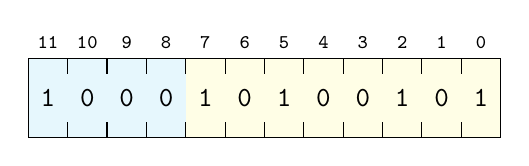
\begin{tikzpicture}
        \fill[cyan!10](0,0) rectangle (2,1);
        \fill[yellow!10](2,0) rectangle (6,1);
        \draw (0,0) rectangle (6,1);
        \foreach \u in {0.5,1.0,...,5.5}
            {
                \draw (\u,0)--(\u,0.2);
                \draw (\u,1)--(\u,0.8);
            }
        \foreach \u in {0,1,...,11}
            {
                \node[above] at (6 - 0.25 - \u * 0.5 ,1){\scriptsize\ttfamily \u};
            }
        \foreach \u \v in {2.25/1,2.75/0,3.25/1,3.75/0,4.25/0,4.75/1,5.25/0,5.75/1,0.25/1,0.75/0,1.25/0,1.75/0}
        \node at (\u,0.5) {\ttfamily \v};
    \end{tikzpicture}
\end{wrapfigure}
資料\cite{armasm}によると,ARMデータの処理命令ビットレイアウトで,即値に当てられているのは下位12ビットのみである.\par
さらに,12ビットの即値を12ビットの番号として処理するのではなく,4ビットの回転値と8ビットの値として処理する(\ref{fig:即値の利用}).
この回転値\(r\)は即値\(I\)を右へ\(2r\)ローテートするために用いる.\par
仮に\(i=\){\ttfamily\ 0x00D30000}が入力されたとする.\(i\)のビット列と右ローテートを\ref{fig:ex}に示す.\(i\)はそのままだと即値として利用できないため,即値として利用できる下位8ビット\(I\)にローテートさせる.(シフトではない.)
このとき16ビットシフトさせたのでこの値を2で割った8を回転数\(r\)に格納し,下位12ビットのみで23ビット必要である数値\(i=\){\ttfamily\ 0x00D30000}を\ref{fig:結果}のように表すことができる.\par
\begin{figure}[H]
    \centering
    \caption{\(i\)のビット列,右ローテート}
    \label{fig:ex}
    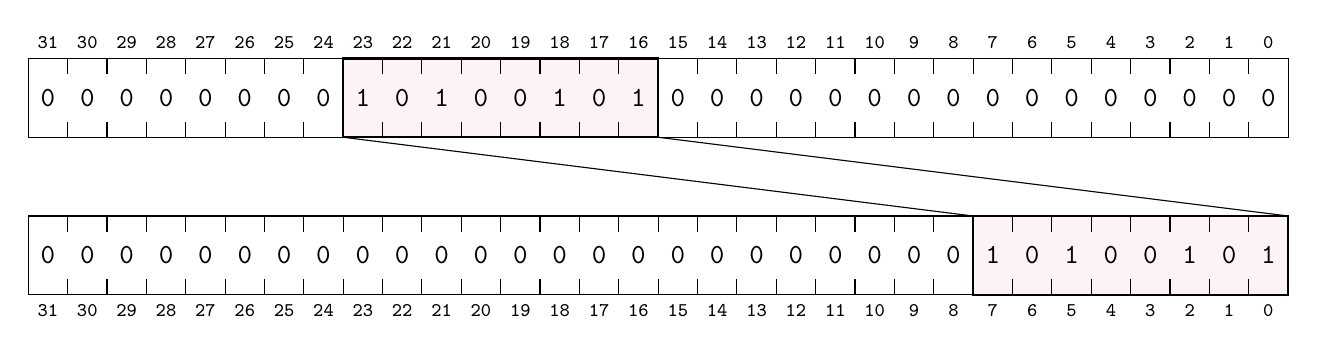
\begin{tikzpicture}[remember picture]
        \fill[fill=magenta!10,opacity=.5](4,0)rectangle(8,1);
        \draw[thick](4,0)rectangle(8,1);
        \draw (0,0) rectangle (16,1);
        \foreach \u in {0.5,1.0, ..., 16.0}
        \draw (\u,0)--(\u,0.2);
        \foreach \u in {0.5,1.0, ..., 16.0}
        \draw (\u,1)--(\u,0.8);
        \foreach \u in {4.25,5.25,6.75,7.75}
        \node at (\u,0.5){{\ttfamily 1}};
        \foreach \u in {4.75,5.75,6.25,7.25}
        \node at (\u,0.5){{\ttfamily 0}};
        \foreach \u in {0.25,0.75,...,3.75}
        \node at (\u,0.5){{\ttfamily 0}};
        \foreach \u in {0,1,...,31}
            {
                \node[above] at (16 - 0.25 - \u * 0.5 ,1){\scriptsize\ttfamily \u};
            }
        \foreach \u in {15.75,15.25,...,8.25}
        \node at (\u,0.5){{\ttfamily 0}};
        \coordinate (S) at (8,0);
        \coordinate (G) at (4,0);
        \fill[fill=magenta!10,opacity=.5](12,-1)rectangle(16,-2);
        \draw[thick](12,-1)rectangle(16,-2);
        \draw (0,-1) rectangle (16,-2);
        \foreach \u in {0.5,1.0, ..., 16.0}
        \draw (\u,-1)--(\u,-1.2);
        \foreach \u in {0.5,1.0, ..., 16.0}
        \draw (\u,-2)--(\u,-1.8);
        \foreach \u in {15.75,14.75,13.25,12.25}
        \node at (\u,-1.5){{\ttfamily 1}};
        \foreach \u in {15.25,14.25,13.75,12.75}
        \node at (\u,-1.5){{\ttfamily 0}};
        \foreach \u in {0.25,0.75,...,11.75}
        \node at (\u,-1.5){{\ttfamily 0}};
        \foreach \u in {0,1,...,31}
            {
                \node[below] at (16 - 0.25 - \u * 0.5 ,-2){\scriptsize\ttfamily \u};
            }
        \coordinate (G2) at (12,-1);
        \coordinate (S2) at (16,-1);
        \draw(G)--(G2);
        \draw(S)--(S2);
    \end{tikzpicture}
\end{figure}
\paragraph{このような設計になっている理由} ARMデータ処理命令のビットレイアウト\cite{armasm}によると,1つのレジスタ内に{\ttfamily Cond}や,加減算,移動,比較などを正確に定義するための値も格納されている.32ビット全てを即値に当てることができず,より少ないビット数でより多くの数値を表現するために,このような設計になったのだろう.
この設計においての不都合は,幾つかの即値を{\ttfamily mov}命令において代入できないことだが,\(2^n(n\in\mathbb{N},0\leq n\leq 31)\)や,32ビット・ワード内の任意の4バイトの位置にあるバイト値の代入を保証しており,最も一般的なケースをカバーしているので使用上の問題は少ないと言える.\cite[p.52]{armprocesser}